% =====================================================================
\chapter{Resultados y Discusión}
\label{cap:resultados}

Los resultados se presentan en el orden de la pregunta. Primero, qué dirección aparece en el
VAR y en las pruebas de Granger (sección~\ref{sec:res-u6}); después, la prueba más favorable a
la hipótesis, con las notas publicadas con el mercado cerrado (sección~\ref{sec:res-u6b});
luego, los estudios de eventos con las dos definiciones de shock
(secciones~\ref{sec:res-u7} y~\ref{sec:res-u7b}); la robustez (sección~\ref{sec:res-u8}) y,
por último, la discusión con la literatura (sección~\ref{sec:discusion}). En todas las tablas,
«significativo» quiere decir significativo al 5\% después de la corrección de
Benjamini-Hochberg.

% ---------------------------------------------------------------------
\section{¿Quién anticipa a quién? VAR y causalidad de Granger}
\label{sec:res-u6}

\subsection{El mercado}

De las ocho pruebas del VAR del mercado, una sola es significativa, y es fuerte: el retorno
del S\&P~Merval anticipa el tono de las noticias ($p$ corregido 0,0003). Ninguna prueba en la
dirección de las noticias hacia el mercado llega a ser significativa, tampoco la de la atención
de los medios hacia el volumen operado (tabla~\ref{tab:u6-mercado}).

\begin{table}[H]
\centering\small
\begin{tabular}{@{}llccc@{}}
\toprule
\textbf{Prueba} & \textbf{Dirección} & \textbf{p} & \textbf{p corregido} & \textbf{Significativo} \\
\midrule
tono \flecha{} retorno & Noticias \flecha{} mercado & 0,2119 & 0,4238 & No \\
retorno \flecha{} tono & Mercado \flecha{} noticias & $<$0,0001 & 0,0003 & \textbf{Sí} \\
tono \flecha{} volumen & Noticias \flecha{} mercado & 0,0632 & 0,2528 & No \\
volumen \flecha{} tono & Mercado \flecha{} noticias & 0,3617 & 0,4823 & No \\
atención \flecha{} retorno & Noticias \flecha{} mercado & 0,9293 & 0,9293 & No \\
retorno \flecha{} atención & Mercado \flecha{} noticias & 0,1479 & 0,3944 & No \\
atención \flecha{} volumen & Noticias \flecha{} mercado & 0,3377 & 0,4823 & No \\
volumen \flecha{} atención & Mercado \flecha{} noticias & 0,5918 & 0,6764 & No \\
\bottomrule
\end{tabular}
\caption{Pruebas de causalidad de Granger en el VAR del mercado (224 ruedas). Fuente:
elaboración propia (\carpeta{Unión/06_var_granger}).}
\label{tab:u6-mercado}
\end{table}

La impulso-respuesta dimensiona el efecto (figura~\ref{fig:irf}). Un día en que el
S\&P~Merval sube un desvío (2,8\%), el tono anormal de las noticias sube 1,84 puntos en la
rueda siguiente y 1,23 en la segunda, ambos distintos de cero; a la tercera (0,56) ya no se
distingue de cero. Como un desvío del tono anormal son 6,0 puntos, la suba de la rueda
siguiente es de un tercio de desvío. El tono y el retorno de una misma rueda también se mueven
juntos (correlación de las sorpresas: 0,19). La impulso-respuesta atribuye ese movimiento
conjunto a las noticias, pero solo porque se las ordenó primero: con datos diarios no se puede
saber quién movió a quién dentro de la rueda. Desde la rueda siguiente, el efecto del tono
sobre el retorno ya no se distingue de cero.

\begin{figure}[H]
\centering
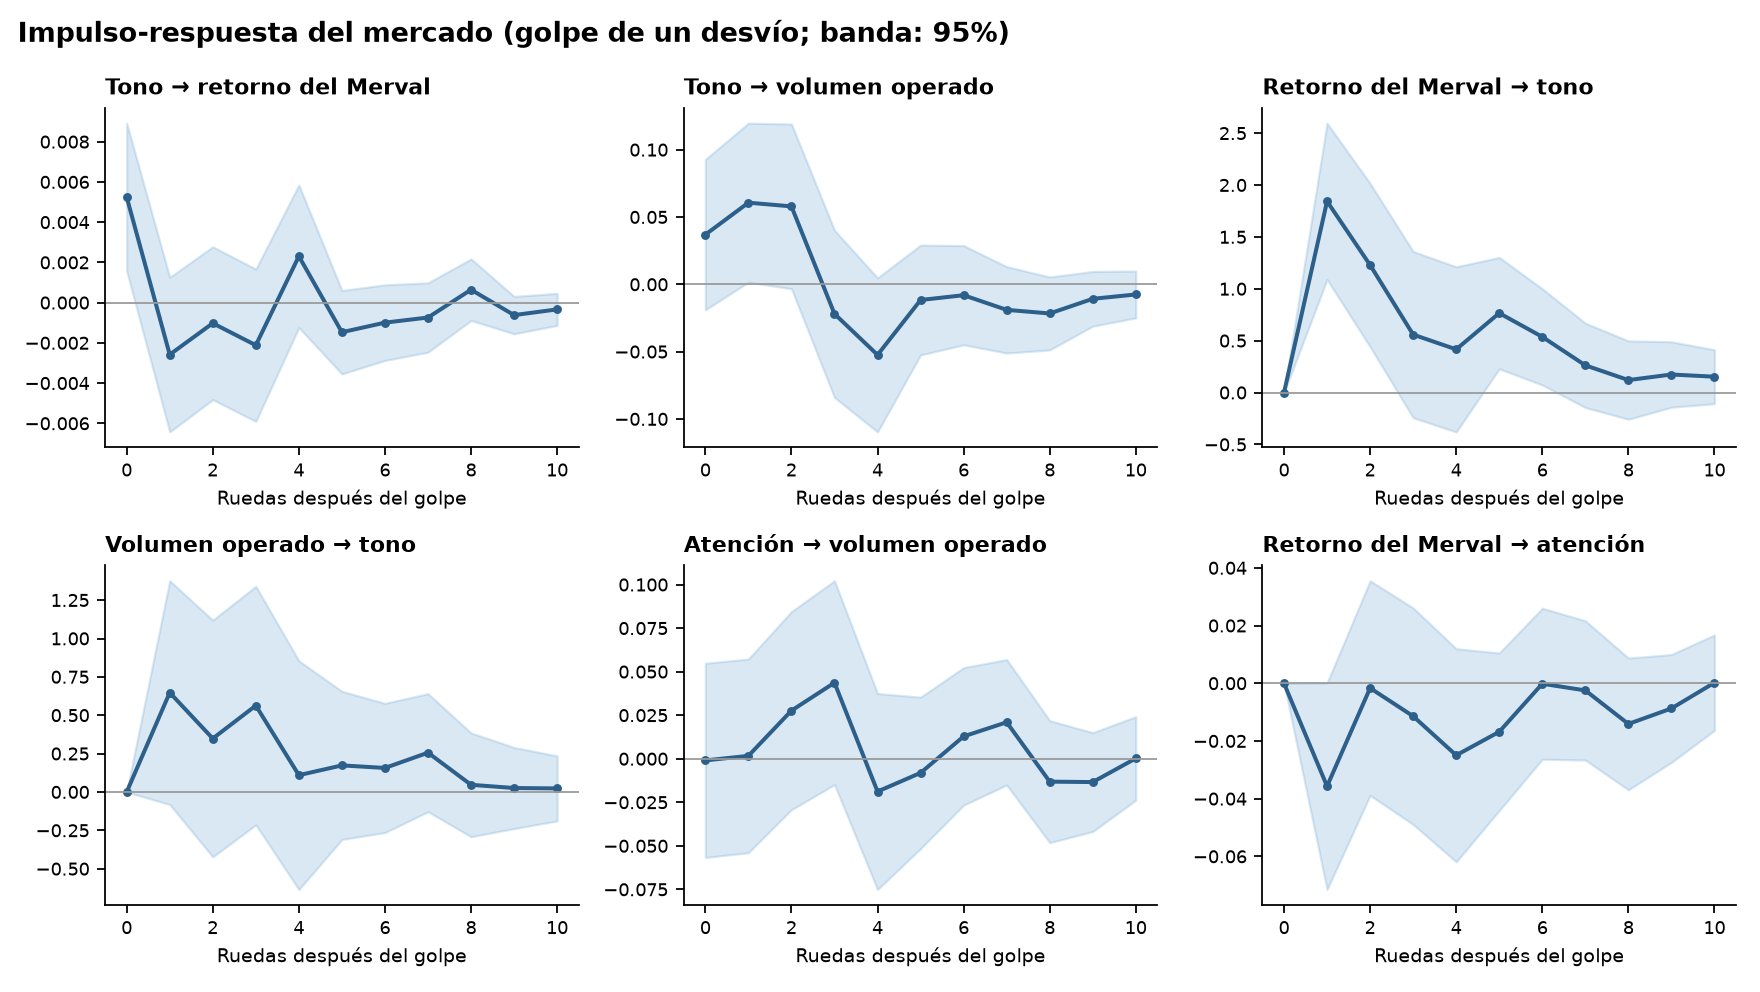
\includegraphics[width=\linewidth]{u6_irf_mercado.png}
\caption{Funciones de impulso-respuesta del VAR del mercado ante un golpe de un desvío, con
banda del 95\%. Si la banda no toca el cero, la respuesta es distinta de cero. Fuente:
elaboración propia (\carpeta{Unión/06_var_granger}).}
\label{fig:irf}
\end{figure}

\subsection{Las empresas}

El retorno de casi todas las empresas anticipa el tono de las noticias: 39 de 47, todas con
signo positivo (tabla~\ref{tab:u6-empresas}). Hay que leerlo con cuidado: en este nivel el
tono es el del mercado, y los retornos de las empresas se mueven con el índice, de modo que en
buena parte es el mismo hallazgo del mercado repetido 47 veces. En la dirección contraria, 7 de
94 pruebas dan $p<0{,}05$ sin corregir, cuando por azar se esperarían unas 9,4; después de la
corrección quedan dos (LONG y SUPV, tono \flecha{} volumen), sin un patrón. El detalle por
empresa está en el anexo~\ref{anx:granger}.

\begin{table}[H]
\centering\small
\begin{tabular}{@{}lcccc@{}}
\toprule
\textbf{Prueba} & \textbf{Pruebas} & \textbf{$p<0{,}05$ sin corregir} & \textbf{Significativas} & \textbf{Signo} \\
\midrule
\multicolumn{5}{@{}l}{\textit{47 empresas, con el tono del mercado}} \\
tono \flecha{} retorno & 47 & 1 & 0 & — \\
tono \flecha{} volumen & 47 & 6 & 2 & 2 positivas \\
retorno \flecha{} tono & 47 & 43 & \textbf{39} & 39 positivas \\
volumen \flecha{} tono & 47 & 11 & 3 & 3 positivas \\
\midrule
\multicolumn{5}{@{}l}{\textit{17 empresas, con su tono propio}} \\
tono propio \flecha{} retorno & 17 & 0 & 0 & — \\
tono propio \flecha{} volumen & 17 & 2 & 1 & 1 positiva \\
retorno \flecha{} tono propio & 17 & 16 & \textbf{15} & 15 positivas \\
volumen \flecha{} tono propio & 17 & 1 & 0 & — \\
\bottomrule
\end{tabular}
\caption{Pruebas de Granger por empresa. Fuente: elaboración propia
(\carpeta{Unión/06_var_granger}).}
\label{tab:u6-empresas}
\end{table}

La prueba más exigente es la del tono propio, que descuenta el clima general de las noticias.
En 15 de las 17 empresas, cuando la acción sube, en las ruedas siguientes se habla de ella
mejor que del resto del mercado: BBAR, BMA, BYMA, CEPU, CRES, EDN, GGAL, IRSA, LOMA, METR, SUPV,
TGSU2, TRAN, TXAR e YPFD. No aparece en ALUA ni en PAMP. Es el resultado más fuerte de la
tesina, porque es específico de cada empresa. En la dirección contraria queda una sola prueba
significativa (IRSA, tono propio \flecha{} volumen), aislada: el tono propio no anticipa ni el
retorno ni el volumen.

\begin{figure}[H]
\centering
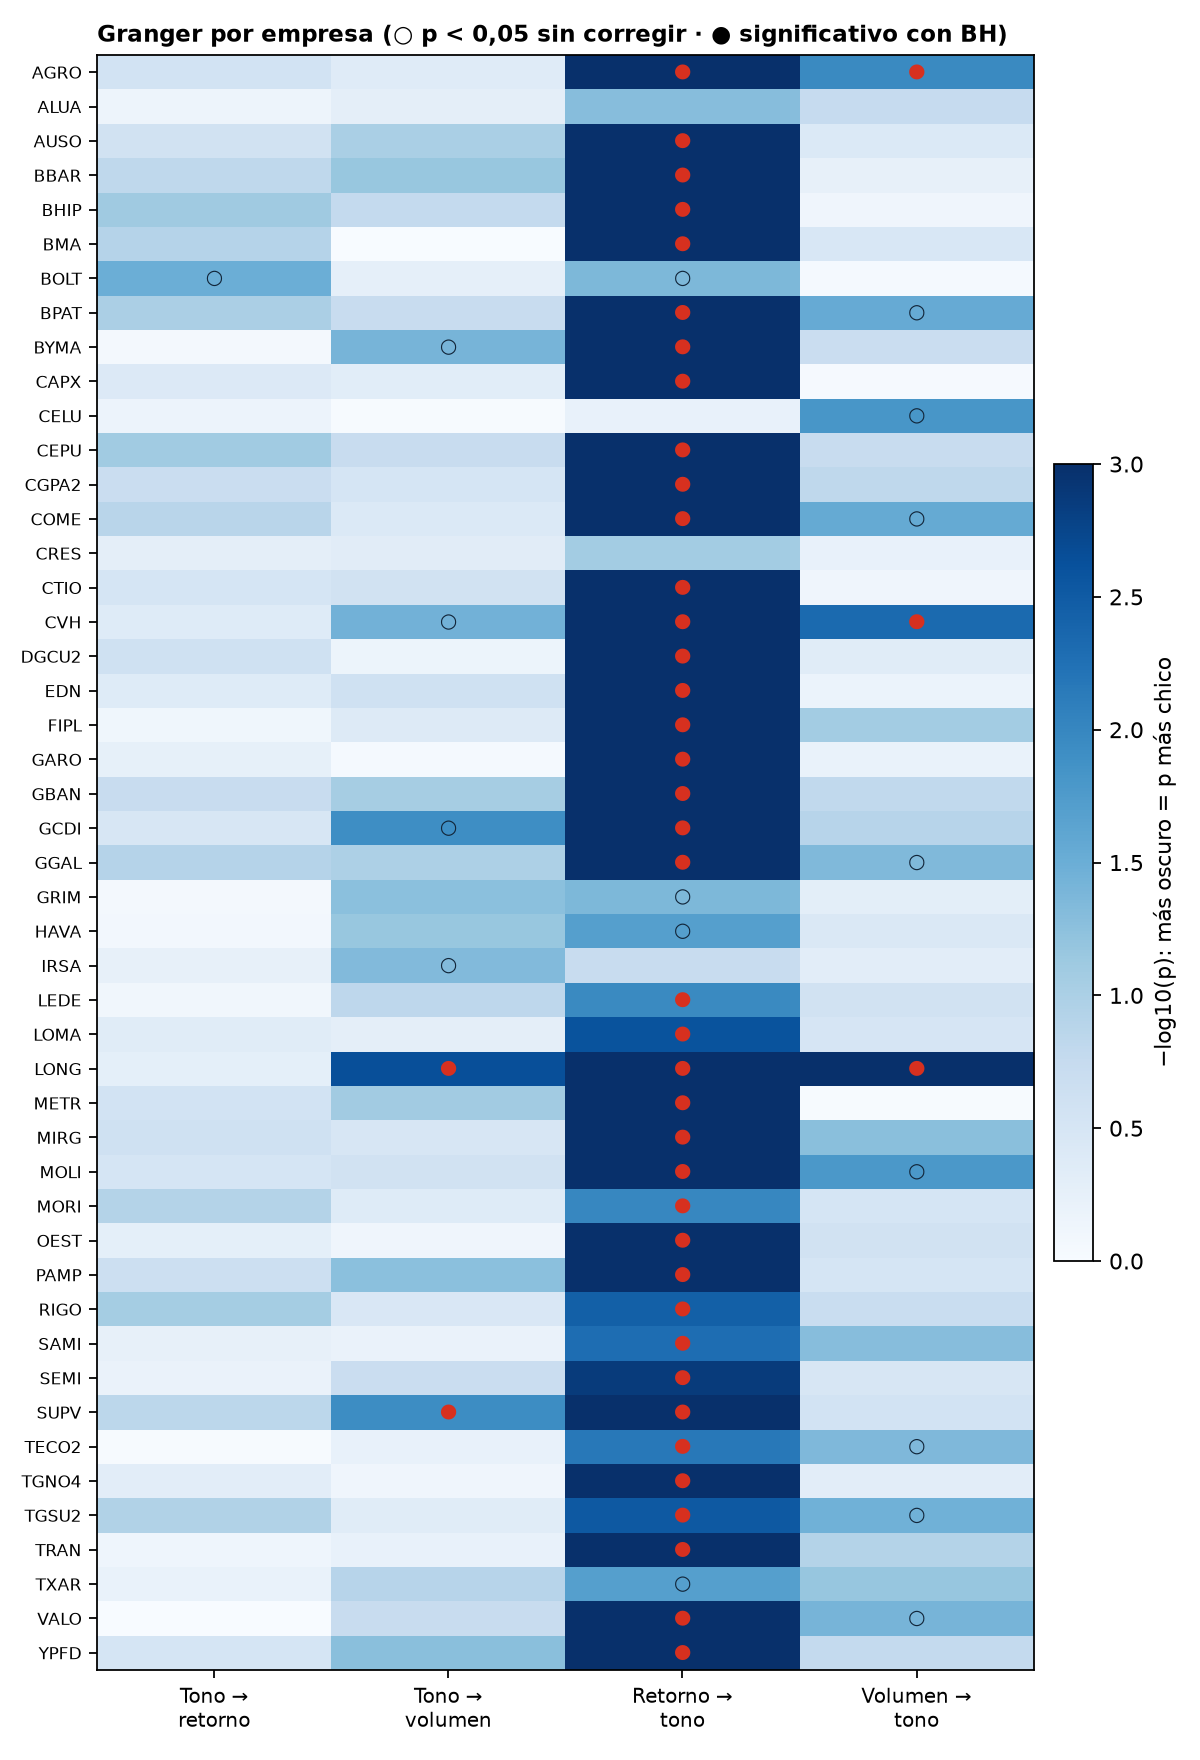
\includegraphics[width=0.58\linewidth]{u6_empresas.png}
\caption{Pruebas de Granger por empresa. Cada fila es una empresa y cada columna una prueba;
más oscuro, $p$ más chico; $\circ$ $p<0{,}05$ sin corregir; $\bullet$ significativo después
de la corrección. Fuente: elaboración propia (\carpeta{Unión/06_var_granger}).}
\label{fig:u6-empresas}
\end{figure}

\subsection{Los sectores y el régimen}

El retorno anticipa el tono en 9 de los 10 sectores; la excepción es Tecnología, que tiene una
sola acción (BOLT). En la otra dirección, solo en Conglomerado el tono anticipa el volumen, y
con signo negativo: un resultado aislado. Sumando todos los niveles, de las 152 pruebas en la
dirección noticias \flecha{} mercado solo 4 son significativas, lo esperable por azar.

\begin{table}[H]
\centering\small
\begin{tabular}{@{}lccc@{}}
\toprule
\textbf{Prueba} & \textbf{Días Calmo} & \textbf{Días Tenso} & \textbf{Diferencia} \\
\midrule
tono \flecha{} retorno & 0,2721 & 0,8436 & 0,9516 \\
tono \flecha{} volumen & 0,0498 & 0,2778 & 0,2810 \\
retorno \flecha{} tono & \textbf{0,0011} & \textbf{0,0006} & 0,6762 \\
volumen \flecha{} tono & 0,4521 & \textbf{0,0021} & 0,0496 \\
\bottomrule
\end{tabular}
\caption{Pruebas de Granger según el régimen ($p$; en negrita, significativas después de la
corrección). Fuente: elaboración propia (\carpeta{Unión/06_var_granger}).}
\label{tab:u6-regimen}
\end{table}

El retorno anticipa el tono tanto en los días Calmo como en los Tenso, sin diferencia entre
ellos (tabla~\ref{tab:u6-regimen}). El volumen anticipa el tono solo en los días Tenso, pero la
diferencia con los Calmo no es significativa tras la corrección; con 40 días Tenso, es poco
para afirmar diferencias entre regímenes. En ningún régimen el tono anticipa al mercado. La
prueba de calibración, con el tono mezclado al azar, dio $p<0{,}05$ en el 6,9\% de los casos,
cerca del 5\% esperado: el test no inventa resultados.

% ---------------------------------------------------------------------
\section{La prueba más directa: notas publicadas con el mercado cerrado}
\label{sec:res-u6b}

El tono de las 8.069 notas publicadas con el mercado cerrado va en la dirección de la
hipótesis: con notas de la noche más positivas, el mercado abre algo más arriba (0,18\% por
cada desvío del tono, cuando el retorno de apertura promedio varía 1,1\% de un día a otro). Pero
no llega a ser significativo: $p=0{,}107$ en el mercado y $0{,}105$ en el panel de empresas
(tabla~\ref{tab:u6b}). Sin los dos días electorales, el efecto del mercado se achica a 0,06\% y
el de las empresas a 0,02\%. Durante la sesión no hay nada. Por empresa, 1 de 34 pruebas da
$p<0{,}05$ sin corregir y ninguna después de la corrección. La calibración con el tono mezclado
al azar dio 4,7\% de $p<0{,}05$.

\begin{table}[H]
\centering\small
\begin{tabular}{@{}llllcc@{}}
\toprule
\textbf{Muestra} & \textbf{Nivel} & \textbf{Retorno} & \textbf{Efecto por desvío} & \textbf{p} & \textbf{p corregido} \\
\midrule
Todas las ruedas & Mercado & Apertura & +0,181\% & 0,107 & 0,213 \\
Todas las ruedas & 17 empresas & Apertura & +0,073\% & 0,105 & 0,213 \\
Todas las ruedas & Mercado & Sesión & +0,201\% & 0,267 & 0,356 \\
Todas las ruedas & 17 empresas & Sesión & +0,041\% & 0,656 & 0,656 \\
Sin días electorales & Mercado & Apertura & +0,059\% & 0,154 & 0,534 \\
Sin días electorales & 17 empresas & Apertura & +0,023\% & 0,391 & 0,534 \\
Sin días electorales & Mercado & Sesión & +0,148\% & 0,401 & 0,534 \\
Sin días electorales & 17 empresas & Sesión & +0,016\% & 0,861 & 0,861 \\
\bottomrule
\end{tabular}
\caption{Tono de las notas publicadas con el mercado cerrado y retorno de la rueda siguiente.
Fuente: elaboración propia (\carpeta{Unión/06b_noticias_preapertura}).}
\label{tab:u6b}
\end{table}

\begin{figure}[H]
\centering
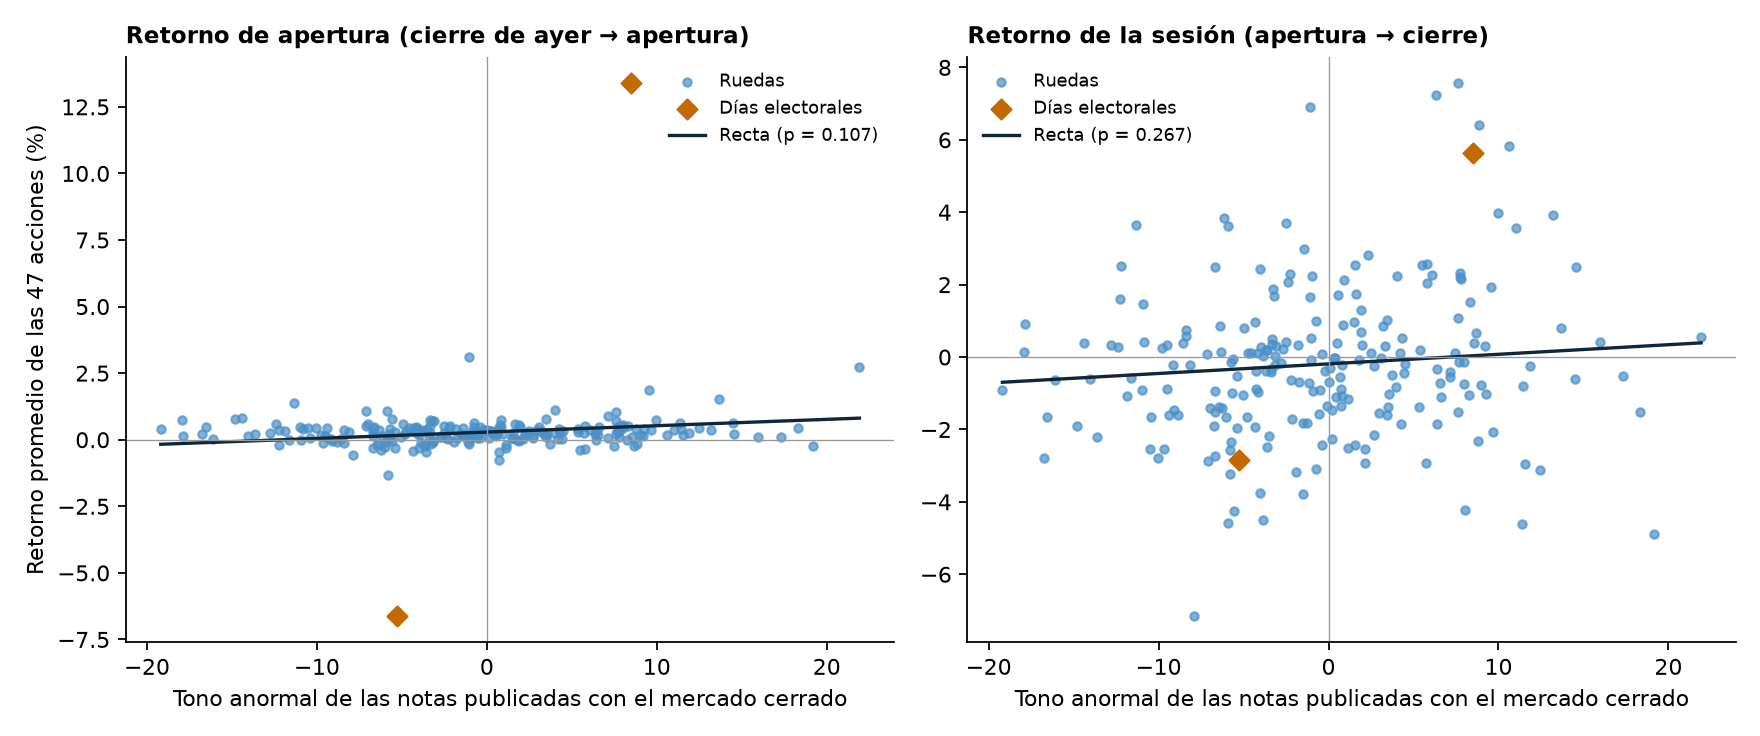
\includegraphics[width=0.95\linewidth]{u6b_preapertura.png}
\caption{Cada punto es una rueda. Horizontal: tono anormal de las notas publicadas con el
mercado cerrado. Vertical: retorno promedio de las 47 acciones, de apertura (izquierda) y de la
sesión (derecha). Fuente: elaboración propia (\carpeta{Unión/06b_noticias_preapertura}).}
\label{fig:u6b}
\end{figure}

Los dos días electorales son exactamente el caso que plantea la hipótesis: noticias de la
noche muy negativas o muy positivas y una apertura que salta en la misma dirección
(tabla~\ref{tab:electorales}). Pero lo que mueve al mercado ahí es el resultado de la elección,
no el tono con que los medios lo cuentan. Fuera de esos dos días, el tono de la noche casi no
se relaciona con la apertura. En cambio, el tono de esas mismas notas se relaciona fuerte con
cómo cerró el mercado el día anterior (correlación 0,42): es el resultado del VAR visto desde
otro ángulo.

\begin{table}[H]
\centering\footnotesize
\begin{tabular}{@{}lcccc@{}}
\toprule
\textbf{Rueda} & \textbf{Notas de la noche} & \textbf{Tono anormal} & \textbf{Apertura} & \textbf{Sesión} \\
\midrule
08/09/2025 (tras las bonaerenses) & 66 & $-$5,3 & $-$6,6\% & $-$2,8\% \\
27/10/2025 (tras las legislativas) & 81 & +8,5 & +13,4\% & +5,6\% \\
\bottomrule
\end{tabular}
\caption{Los dos días electorales en la prueba pre-apertura. Fuente: elaboración propia
(\carpeta{Unión/06b_noticias_preapertura}).}
\label{tab:electorales}
\end{table}

% ---------------------------------------------------------------------
\section{Estudio de eventos: ruedas de tono extremo}
\label{sec:res-u7}

En las ruedas de tono extremo positivo, el S\&P~Merval sube 2,01\% el mismo día, en los 7
eventos ($p$ del test $t$ 0,009; contra fechas al azar, 0,018). Y ya venía subiendo: +3,19\%
en las tres ruedas previas (contra el azar, $p=0{,}037$). Después del evento no pasa nada
($-2{,}80\%$, indistinguible del azar). En las ruedas de tono extremo negativo no aparece ningún
movimiento (tabla~\ref{tab:u7}). El monto operado acompaña al precio: en los eventos positivos
ya estaba 0,24 por encima de lo habitual en las tres ruedas previas (contra el azar,
$p=0{,}031$) y vuelve a lo normal después. Dejando solo el primero de cada grupo de eventos
solapados quedan 4 eventos positivos, y la suba del día se mantiene (+2,40\%, $p=0{,}034$
contra el azar).

\begin{table}[H]
\centering\small
\begin{tabular}{@{}llcccc@{}}
\toprule
\textbf{Eventos} & \textbf{Tramo} & \textbf{CAR medio} & \textbf{Con suba} & \textbf{p (test t)} & \textbf{p (azar)} \\
\midrule
Positivos (7) & Antes $[-3,-1]$ & +3,19\% & 5 de 7 & 0,188 & \textbf{0,037} \\
 & Día $[0]$ & +2,01\% & 7 de 7 & \textbf{0,009} & \textbf{0,018} \\
 & Después $[+1,+5]$ & $-$2,80\% & 3 de 7 & 0,345 & 0,306 \\
\midrule
Negativos (9) & Antes $[-3,-1]$ & $-$0,84\% & 4 de 9 & 0,633 & 0,645 \\
 & Día $[0]$ & $-$0,01\% & 4 de 9 & 0,988 & 0,915 \\
 & Después $[+1,+5]$ & +1,27\% & 5 de 9 & 0,420 & 0,370 \\
\bottomrule
\end{tabular}
\caption{Retorno anormal acumulado del S\&P~Merval alrededor de las ruedas de tono extremo.
Fuente: elaboración propia (\carpeta{Unión/07_event_study}).}
\label{tab:u7}
\end{table}

\begin{figure}[H]
\centering
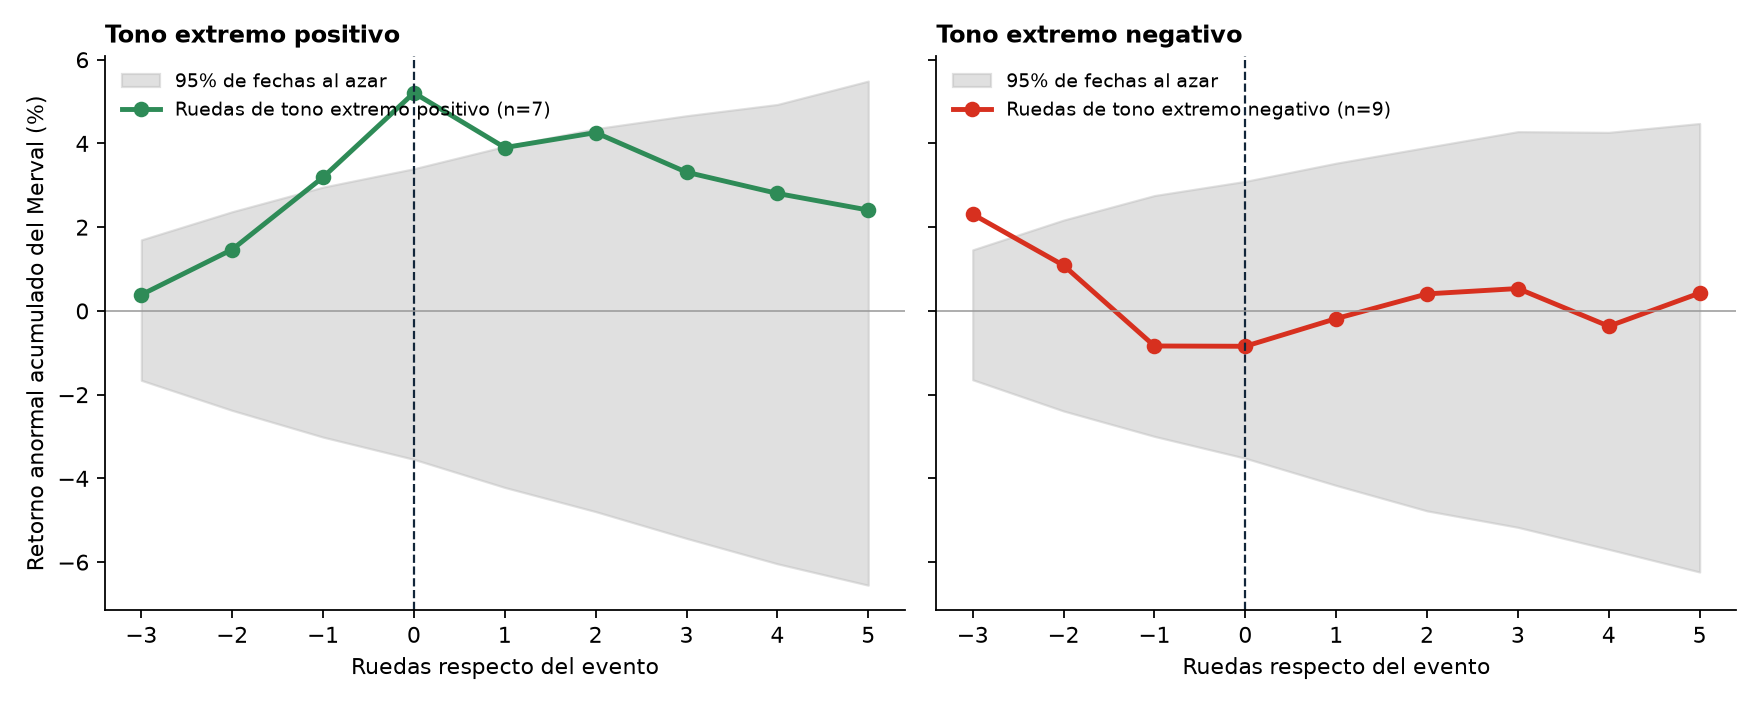
\includegraphics[width=0.95\linewidth]{u7_mercado.png}
\caption{Retorno anormal acumulado promedio del S\&P~Merval desde tres ruedas antes hasta
cinco después de las ruedas de tono extremo. La banda gris es el 95\% de lo que da el azar con
la misma cantidad de fechas. Fuente: elaboración propia (\carpeta{Unión/07_event_study}).}
\label{fig:u7}
\end{figure}

Con las empresas ocurre lo mismo. Cuando se habla de una empresa de forma muy positiva, su
acción ya había subido 1,24\% más que el mercado en las tres ruedas previas (62 eventos,
$p=0{,}029$), y después no pasa nada ($-0{,}14\%$). Con el tono muy negativo, la acción venía
de bajar 2,12\% ($p=0{,}061$) y después rebota 2,96\% ($p=0{,}099$), sin llegar al 5\%. El
volumen de la empresa no cambia (figura~\ref{fig:u7-empresa}).

\begin{figure}[H]
\centering
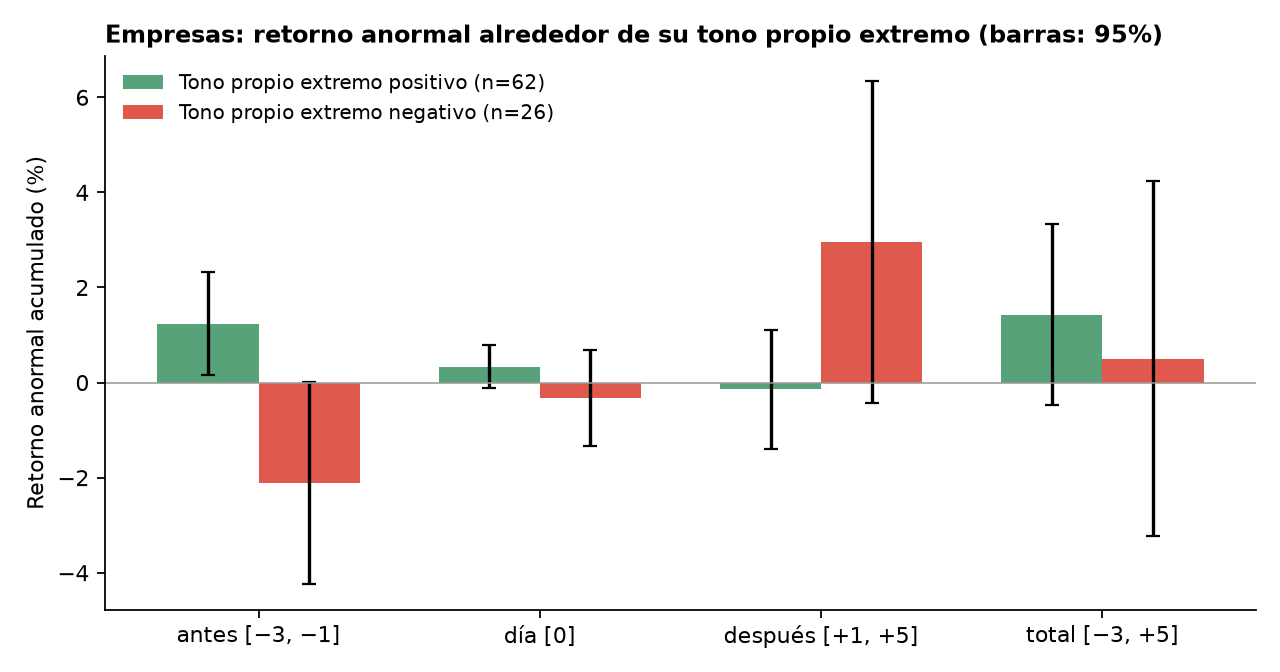
\includegraphics[width=0.7\linewidth]{u7_empresa.png}
\caption{Retorno anormal acumulado de cada empresa alrededor de sus ruedas de tono propio
extremo, positivo y negativo. Fuente: elaboración propia (\carpeta{Unión/07_event_study}).}
\label{fig:u7-empresa}
\end{figure}

El estudio de eventos cuenta la misma historia que el VAR: el precio y el volumen se mueven
antes o junto con las noticias extremas, no después. Las ruedas de tono muy positivo son ruedas
de suba del mercado; pasada esa rueda, el tono no deja nada por anticipar. El efecto aparece
con el tono positivo y no con el negativo, pero con 7 y 9 eventos no se puede afirmar que la
asimetría sea real.

% ---------------------------------------------------------------------
\section{Estudio de eventos: shocks de cantidad de noticias}
\label{sec:res-u7b}

Con la definición del plan corregida por día de calendario, el mercado tiene 6 eventos y
ninguna medida se distingue de un día cualquiera. En las 17 empresas hay 105 shocks
(tabla~\ref{tab:u7b}). El volumen anormal del día del shock es claramente mayor que en un día
cualquiera (0,139 contra $-0{,}054$; $p$ corregido 0,017): cuando una empresa aparece en muchas
más notas que lo habitual, ese día su acción se opera más. El precio se mueve algo más, para un
lado o para el otro (2,02\% en valor absoluto contra 1,61\%; $p$ corregido 0,059), pero el
retorno acumulado no tiene dirección y no hay nada en los días siguientes. Antes del shock no
aparece nada significativo: el precio no viene moviéndose antes de que aumente la cantidad de
noticias.

\begin{table}[H]
\centering\footnotesize
\begin{tabular}{@{}llcccc@{}}
\toprule
\textbf{Nivel} & \textbf{Medida} & \textbf{Shocks} & \textbf{Día cualquiera} & \textbf{p (azar)} & \textbf{p corregido} \\
\midrule
Mercado (6) & $|$RA$|$ día $[0]$ & 2,11\% & 1,83\% & 0,642 & 0,956 \\
 & Vol.\ anormal día $[0]$ & $-$0,003 & $-$0,027 & 0,886 & 0,956 \\
 & CAR día $[0]$ & $-$1,50\% & $-$0,07\% & 0,127 & 0,443 \\
\midrule
Empresas (105) & $|$RA$|$ día $[0]$ & 2,02\% & 1,61\% & 0,008 & 0,059 \\
 & Vol.\ anormal antes $[-3,-1]$ & 0,038 & $-$0,043 & 0,051 & 0,237 \\
 & Vol.\ anormal día $[0]$ & 0,139 & $-$0,054 & 0,001 & \textbf{0,017} \\
 & Vol.\ anormal después $[+1,+5]$ & $-$0,045 & $-$0,052 & 0,849 & 0,956 \\
 & CAR día $[0]$ & 0,13\% & 0,01\% & 0,591 & 0,956 \\
 & CAR después $[+1,+5]$ & $-$0,02\% & 0,06\% & 0,905 & 0,956 \\
\bottomrule
\end{tabular}
\caption{Estudio de eventos de los shocks de cantidad de noticias (selección de las 14
pruebas principales; el resto no es significativo). RA: retorno anormal; Vol.: volumen
anormal en logaritmo (0 = lo habitual). La corrección de Benjamini-Hochberg se aplica sobre
las 14. Fuente: elaboración propia (\carpeta{Unión/07b_shock_volumen_noticias}).}
\label{tab:u7b}
\end{table}

La rueda del shock incluye notas publicadas durante la misma sesión, que pueden estar contando
la suba o la baja del día. Por eso «el precio se mueve más el día del shock» no dice qué vino
primero. La prueba que cuenta solo las notas publicadas con el mercado cerrado lo aclara
(tabla~\ref{tab:u7b-pre}): en las empresas, el salto de apertura no es mayor que en un día
cualquiera (0,82\% contra 0,72\%; $p$ corregido 0,544), aunque el volumen del día tiende a ser
mayor ($p$ corregido 0,053). En el mercado el salto de apertura sí es mayor ($p$ corregido
0,022), pero con 5 eventos y apoyado en un solo día: sin el 24/09/2025, el del anuncio del
Tesoro de Estados Unidos, el promedio baja de 0,95\% a 0,59\% y el $p$ sube a 0,093. Es el
mismo patrón de las elecciones: un hecho grande genera muchas noticias y mueve el precio, pero
lo que mueve al mercado es el hecho, no la cantidad de cobertura.

\begin{table}[H]
\centering\footnotesize
\begin{tabular}{@{}llcccc@{}}
\toprule
\textbf{Nivel} & \textbf{Medida} & \textbf{Shocks} & \textbf{Día cualquiera} & \textbf{p (azar)} & \textbf{p corregido} \\
\midrule
Mercado (5) & $|$Salto de apertura anormal$|$ & 0,95\% & 0,33\% & 0,004 & 0,022 \\
 & $|$RA$|$ día $[0]$ & 1,64\% & 1,83\% & 0,790 & 0,875 \\
 & Vol.\ anormal día $[0]$ & $-$0,057 & $-$0,027 & 0,875 & 0,875 \\
\midrule
Empresas (76) & $|$Salto de apertura anormal$|$ & 0,82\% & 0,72\% & 0,293 & 0,544 \\
 & $|$RA$|$ día $[0]$ & 1,77\% & 1,61\% & 0,363 & 0,544 \\
 & Vol.\ anormal día $[0]$ & 0,105 & $-$0,054 & 0,018 & 0,053 \\
\bottomrule
\end{tabular}
\caption{Shocks de cantidad contando solo las notas publicadas con el mercado cerrado. El
salto de apertura del mercado depende del 24/09/2025: sin ese día, $p=0{,}093$. Fuente:
elaboración propia (\carpeta{Unión/07b_shock_volumen_noticias}).}
\label{tab:u7b-pre}
\end{table}

\begin{figure}[H]
\centering
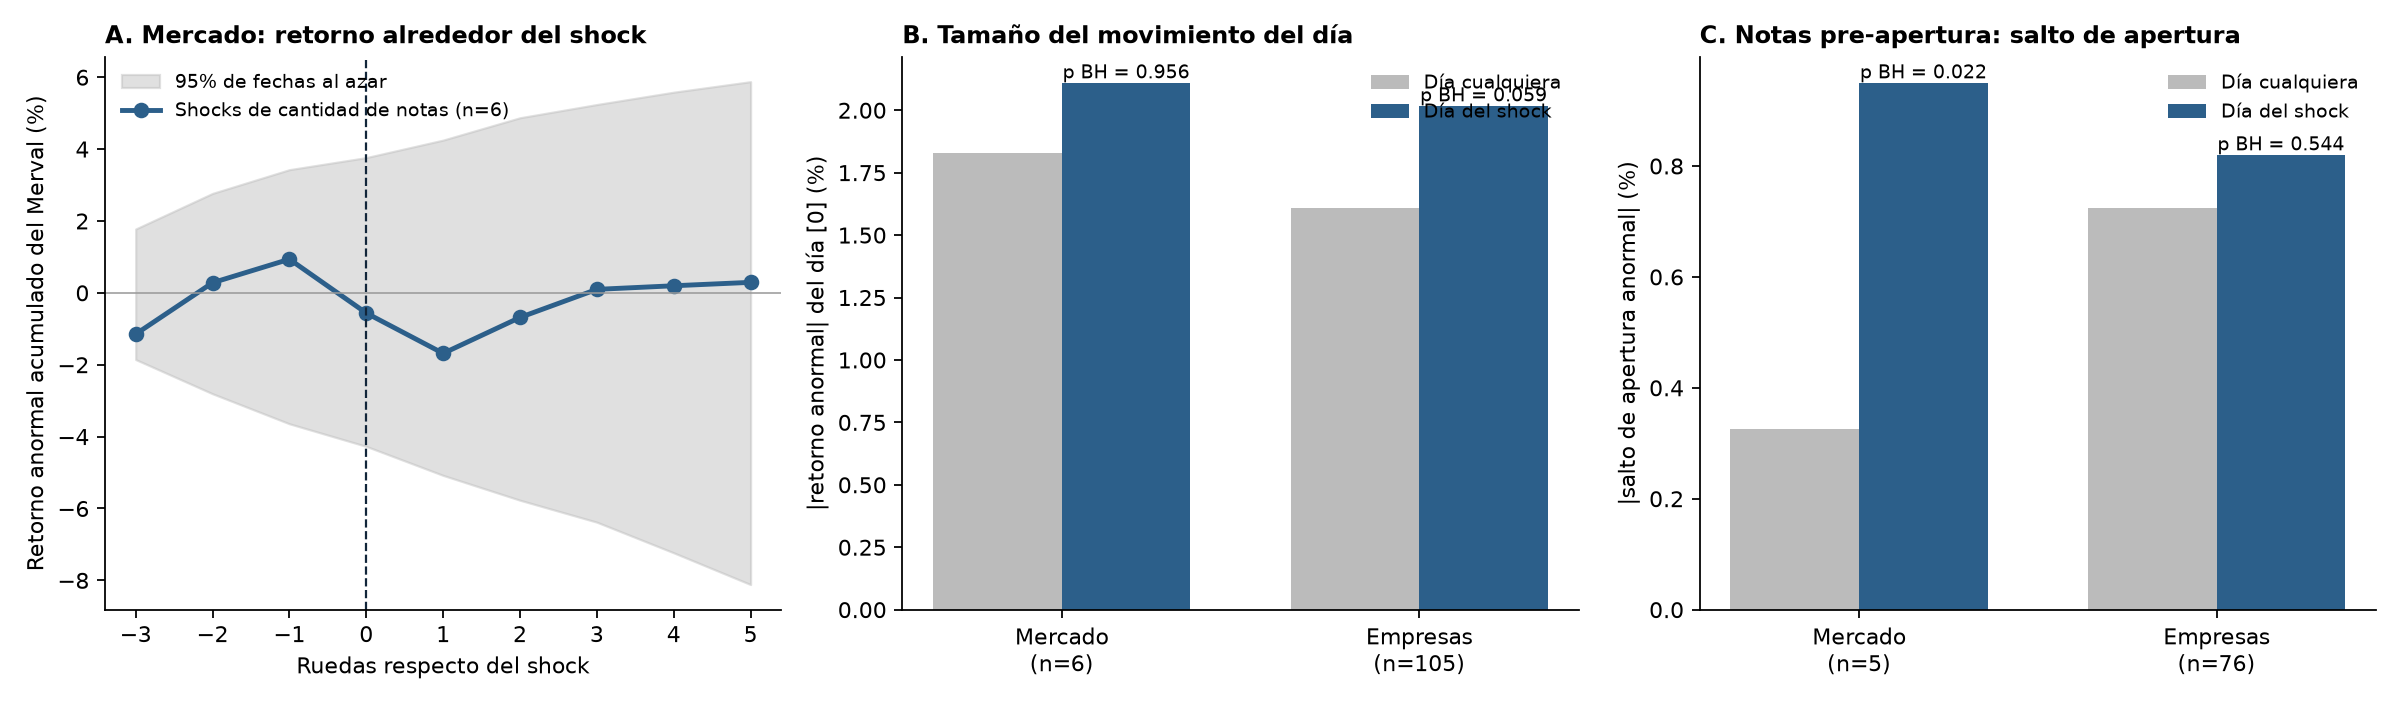
\includegraphics[width=\linewidth]{u7b_shock_volumen.png}
\caption{A: retorno anormal acumulado del S\&P~Merval alrededor de los shocks de cantidad,
contra el 95\% de fechas al azar. B y C: tamaño del movimiento en los shocks contra un día
cualquiera; C cuenta solo las notas publicadas con el mercado cerrado. Fuente: elaboración
propia (\carpeta{Unión/07b_shock_volumen_noticias}).}
\label{fig:u7b}
\end{figure}

Los análisis secundarios confirman que el resultado de las empresas no depende de una decisión
puntual: el movimiento y el volumen del día son mayores con umbral $z>2{,}5$ (70 eventos), con
el puntaje $z$ sobre $\log(1+\text{cantidad})$ (63 eventos) y sumando los eventos con una
elección en su ventana (114). Separando por el tono de la rueda, el efecto aparece en los shocks
de tono negativo (46 eventos) y no en los de tono positivo (59). En la versión original, sin
dividir por los días que cubre la rueda, los 12 eventos del mercado son todas ruedas posteriores
a un día sin mercado y no muestran nada; en las empresas, el resultado del volumen es el mismo.

Según la regla fijada antes de correr la prueba, el volumen anormal del día del shock en las
empresas cuenta como evidencia a favor de H1, y es significativo tras la corrección. La
hipótesis encuentra, entonces, un \textit{apoyo parcial, en el volumen}: cuando una empresa
está en muchas más notas, ese día se opera más. No hay un efecto con dirección sobre el precio,
ni arrastre en los días siguientes, y las notas de la noche no anticipan la apertura.

% ---------------------------------------------------------------------
\section{Robustez: cuándo siguen los medios al mercado}
\label{sec:res-u8}

De 106 comparaciones entre la base y las doce variantes, 93 mantienen la conclusión
(tabla~\ref{tab:u8}). Dos resultados se sostienen en todas. Primero, el tono no anticipa al
mercado: en ninguna variante el tono anticipa el retorno, ni en el mercado ni en ninguna
empresa. Es el resultado más firme de la tesina. Segundo, el mercado anticipa al tono con
cualquier medida de tono y sin los días dudosos: con el tono ajustado por portal, con el tono
en nivel, sin las notas de hora sospechosa, sin abril de 2026, con los días electorales como
control y sin las acciones ilíquidas (36 de 43 empresas). Con el régimen filtrado o juntando
Moderado con Tenso, el retorno sigue anticipando el tono en los dos tipos de días. En el estudio
de eventos, la suba del S\&P~Merval en las ruedas de tono extremo positivo se mantiene con el
umbral 3, que deja solo las cuatro más extremas (+1,50\%, $p=0{,}038$), con el umbral 2
(+2,42\%, $p=0{,}009$) y sin las notas de hora sospechosa (+1,95\%, $p=0{,}025$).

\begin{table}[H]
\centering\footnotesize
\begin{tabular}{@{}L{4.3cm}C{1.65cm}C{1.65cm}C{1.65cm}C{1.65cm}C{1.65cm}@{}}
\toprule
\textbf{Variante} & \textbf{Ret. \flecha{} tono (p)} & \textbf{Tono \flecha{} ret. (p)} & \textbf{Ret. \flecha{} propio (de 17)} & \textbf{Propio \flecha{} ret. (de 17)} & \textbf{Ret. \flecha{} tono (de 47)} \\
\midrule
Base & 0,0003 & 0,4238 & 15 & 0 & 39 \\
Tono ajustado por portal & 0,0003 & 0,4483 & 15 & 0 & 39 \\
Tono en nivel & 0,0002 & 0,4752 & 11 & 0 & 34 \\
Sin notas de hora sospechosa & 0,0002 & 0,4903 & 16 & 0 & 40 \\
Fecha de calendario & 0,3389 & 0,4183 & 0 & 0 & 0 \\
Solo notas del día, antes del cierre & 0,7000 & 0,4450 & 0 & 0 & 0 \\
Sin abril de 2026 & 0,0004 & 0,2239 & 16 & 0 & 39 \\
Días electorales como control & 0,0003 & 0,5602 & 15 & 0 & 38 \\
\bottomrule
\end{tabular}
\caption{Resultados principales en cada variante ($p$ corregidos). Fuente: elaboración propia
(\carpeta{Unión/08_robustez}).}
\label{tab:u8}
\end{table}

Con dos variantes el efecto del retorno sobre el tono desaparece: la fecha de calendario y las
notas del día antes del cierre. Las dos tienen algo en común: dejan afuera, o cambian de rueda,
las notas publicadas después del cierre. Para ver exactamente dónde está el efecto se separaron
las notas según la franja en que se publicaron (tabla~\ref{tab:franjas}).

\begin{table}[H]
\centering\footnotesize
\begin{tabular}{@{}lrcc@{}}
\toprule
\textbf{Franja de publicación} & \textbf{Notas} & \textbf{Efecto de un desvío del retorno} & \textbf{p} \\
\midrule
Noche del día de la rueda (17 a 24 h) & 3.451 & \textbf{+4,77 puntos de tono} & $<$0,0001 \\
Día sin rueda & 2.142 & +3,11 & 0,1133 \\
Madrugada y mañana siguientes (antes de las 11) & 4.331 & +0,54 & 0,5142 \\
Sesión (11 a 17 h) & 4.001 & +1,26 & 0,1028 \\
\bottomrule
\end{tabular}
\caption{Relación entre el retorno de una rueda y el tono de las notas según la franja en que
se publicaron. Fuente: elaboración propia (\carpeta{Unión/08_robustez}).}
\label{tab:franjas}
\end{table}

El efecto está en las notas de la misma noche, publicadas entre las 17:00 y la medianoche del
día de la rueda: un desvío del retorno sube su tono 4,8 puntos. En las notas de la madrugada y
la mañana siguiente es casi nulo. La regla de las 17:00 manda las notas de la noche a la rueda
siguiente, y por eso en el VAR el efecto aparece como «el retorno de hoy anticipa el tono de
mañana». En realidad es más directo: después del cierre, los medios cuentan cómo le fue al
mercado y a cada empresa con un tono que acompaña la suba o la baja, y no hay un arrastre que
dure días. Con el tono propio de cada empresa pasa lo mismo: usando solo las notas del día antes
del cierre, el efecto desaparece en las 17 empresas.

\begin{figure}[H]
\centering
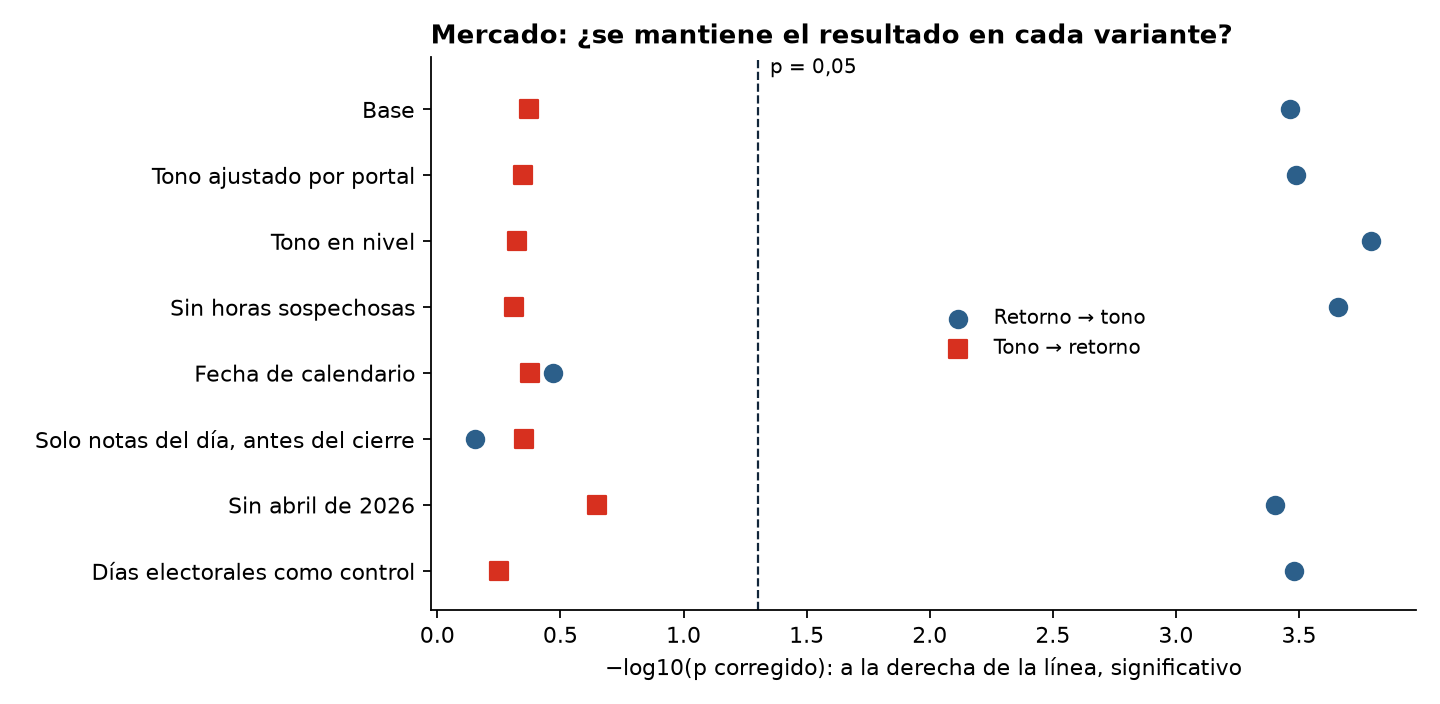
\includegraphics[width=0.88\linewidth]{u8_robustez.png}
\caption{Resultados principales en cada variante de robustez. Fuente: elaboración propia
(\carpeta{Unión/08_robustez}).}
\label{fig:u8}
\end{figure}

% ---------------------------------------------------------------------
\section{Discusión}
\label{sec:discusion}

\textbf{Los medios siguen al mercado.} El resultado central coincide con uno de los dos
hallazgos de \citet{tetlock2007}: los retornos anticipan el tono de la cobertura. Que se repita
con medios argentinos, en otro idioma y con un modelo de sentimiento distinto, lo hace más
creíble. La robustez agrega una precisión que el trabajo de Tetlock, con una columna diaria, no
podía dar: el efecto está en las notas publicadas la misma noche, después del cierre, que cuentan
la jornada. Es consistente con \citet{verma2026}, para quienes buena parte de la cobertura refleja
información que el precio ya incorporó, y con la pregunta de \citet{kargarzadeh2026} sobre en
qué momento una noticia «ya está en el precio»: en las ruedas de tono extremo, el S\&P~Merval ya
venía subiendo antes.

\textbf{Las noticias no anticipan al mercado.} Aquí el resultado difiere de \citet{tetlock2007}
y de \citet{galdi2018}, que encuentran contenido informativo en el tono de los medios de
Estados Unidos y Brasil. La diferencia no contradice a la literatura. \citet{garcia2013} muestra
que el efecto del tono sobre los retornos se concentra en las recesiones, y la ventana de esta
tesina es de un solo año; además, el análisis por régimen no encontró efecto ni siquiera en los
días de mayor estrés del mercado (régimen Tenso). También es compatible con un mercado que incorpora la
información rápido \citep{fama1970}: los hechos grandes —las elecciones, el anuncio del Tesoro
de Estados Unidos— se reflejan de inmediato en la apertura, y el tono con que los medios los
cuentan no agrega información que el precio no tenga. La prueba pre-apertura, la más parecida a
la de \citet{glasserman2025}, encuentra un indicio del signo esperado ($p\approx0{,}1$) que se
apoya en los días electorales.

\textbf{La cantidad de noticias acompaña a la actividad.} Que una empresa con muchas más notas
se opere más ese día está en línea con la literatura de atención \citep{da2011,fang2009,cao2025hype}
y con la evidencia de \citet{engelberg2011} de que la cobertura de medios se asocia con el
volumen operado. A diferencia de \citet{coronado2022,coronado2023}, que encuentran causalidad
desde índices de cantidad de noticias del COVID hacia las bolsas latinoamericanas, aquí la
cantidad no anticipa la apertura de cada empresa: el movimiento del día puede ser tanto la
reacción a la noticia como la noticia contando el movimiento. La relación entre retorno y
volumen, por su parte, es conocida en la región: el retorno tiende a anticipar al volumen
\citep{rojas2015}.

\textbf{Tono por empresa.} El hallazgo más específico —después de que una acción sube, se habla
de esa empresa mejor que del resto— no podría verse con un tono por nota. Respalda medir el
sentimiento a nivel de entidad \citep{tang2023finentity,sinha2023sentfin} y descontar el tono
general del día, una forma de tono anormal como la de \citet{ardia2022}. El encogimiento hacia
el promedio \citep{efron1975,carbo2026} fue necesario porque en muchas ruedas el tono de una
empresa se apoya en una o dos oraciones.

\textbf{Pruebas múltiples y especificaciones previas.} Se hicieron cientos de pruebas. Sin
corrección, algunas habrían salido significativas por azar \citep{harvey2016,harvey2020}; con
ella, la dirección noticias \flecha{} mercado deja 4 de 152 pruebas, lo esperable por azar. Las
dos especificaciones escritas antes de correr y la robustez con una decisión por vez responden
a la advertencia de \citet{nikolopoulos2026} sobre la predictibilidad espuria que aparece al
probar variantes hasta que una funciona. El único cambio posterior (la cantidad por día de
calendario en U7b) quedó documentado con su motivo, y se informan las dos versiones.

\textbf{En la región.} Los trabajos que cruzan tono de medios y precios en Latinoamérica son
pocos \citep{galdi2018,cruzmontana2025} y ninguno es argentino. Las elecciones fueron, como en
\citet{calandroni2026}, los shocks de información más fuertes del período; y, como sugiere
\citet{amburgey2025} para los sectores, el análisis por sector muestra que la dirección mercado
\flecha{} noticias aparece en casi todos, mientras que la contraria aparece de forma aislada
(Conglomerado, con signo negativo).
